\documentclass[sigconf]{acmart}
% Cleaning
\pagestyle{fancy} % removes running headers
\settopmatter{printacmref=false} % Removes citation information below abstract
\renewcommand\footnotetextcopyrightpermission[1]{} % removes footnote with conference information in first column
\pagestyle{plain} % removes running headers
\fancyhead{}
\settopmatter{printacmref=false, printfolios=false}
% Copyright
\setcopyright{none}
% \setcopyright{acmcopyright}
% \setcopyright{acmlicensed}
% \setcopyright{rightsretained}
% \setcopyright{usgov}
% \setcopyright{usgovmixed}
% \setcopyright{cagov}
% \setcopyright{cagovmixed}
\settopmatter{printacmref=false} % Removes citation information below abstract
\acmDOI{}


\setlength{\parskip}{0pt}
\setlength{\parsep}{0pt}
\setlength{\headsep}{0pt}
\setlength{\topskip}{0pt}
\setlength{\topmargin}{0pt}
\setlength{\topsep}{0pt}
\setlength{\partopsep}{0pt}
%\linespread{0.95}
\usepackage{mdwlist}
\usepackage{amsmath}


\begin{document}
\title{SENG 474 Project Proposal}
\author{Parris Mook-Sang-Forbes}
\affiliation{
  \institution{University of Victoria}
}
\email{parrisf@uvic.ca }
\author{Max Patchell}
\affiliation{
  \institution{University of Victoria}
}
\email{maxpatchell@uvic.ca}
\author{Varun Menon}
\affiliation{
  \institution{University of Victoria}
}
\email{varunmenon@uvic.ca}

\begin{abstract}
This project classifies aerial wildfire images into three operational risk tiers, namely low, medium, and high. By training a model to differentiate genuine fire development from confounding environmental variables like fog, weather, terrain, foliage, etc to minimize false positive detections. This ensures that critical firefighting resources are deployed based on actual threats rather than algorithmic errors.
\end{abstract}

\keywords{Artificial Intelligence, Wildfires, Forest Fires, Aerial Photography}
\maketitle

\section{Introduction}
Aerial images can provide visual information about wildfires at different stages of intensity. Interpreting these images can be challenging, as fire and smoke can be hard to differentiate between environmental/weather features like clouds, fog, sunset/sunlight reflections. El-Madafri et al. [2023] identify these same issues as an important issue to pursue in order to make image based wildfire detection more reliable. 

This project investigates the classification of aerial wildfire images into three risk categories; low, medium and high. Given an individual image the objective of our model is to be able to map from visual features to the corresponding risk category, while focusing on having a reduction on misclassifications due to environmental conditions. The specific focus on reducing misclassifications is to account for real world conditions where wasted fire department resources is a serious consequence rather than a slight calculation error. We must be able to differentiate between wildfire photography (Figure 1), and photos with similar elements to the former but containing no wildfires (Figure 2). By examining images at different stages of fire development, the project aims to accurately distinguish the level of apparent risk including the reduction of incorrect assignment of elevated risks due to misleading visual features. 

\begin{figure}[htp]
\caption{An aerial photograph of a wildfire via \emph{Applied Sciences}. (https://doi.org/10.3390/app13148275)}
\centering
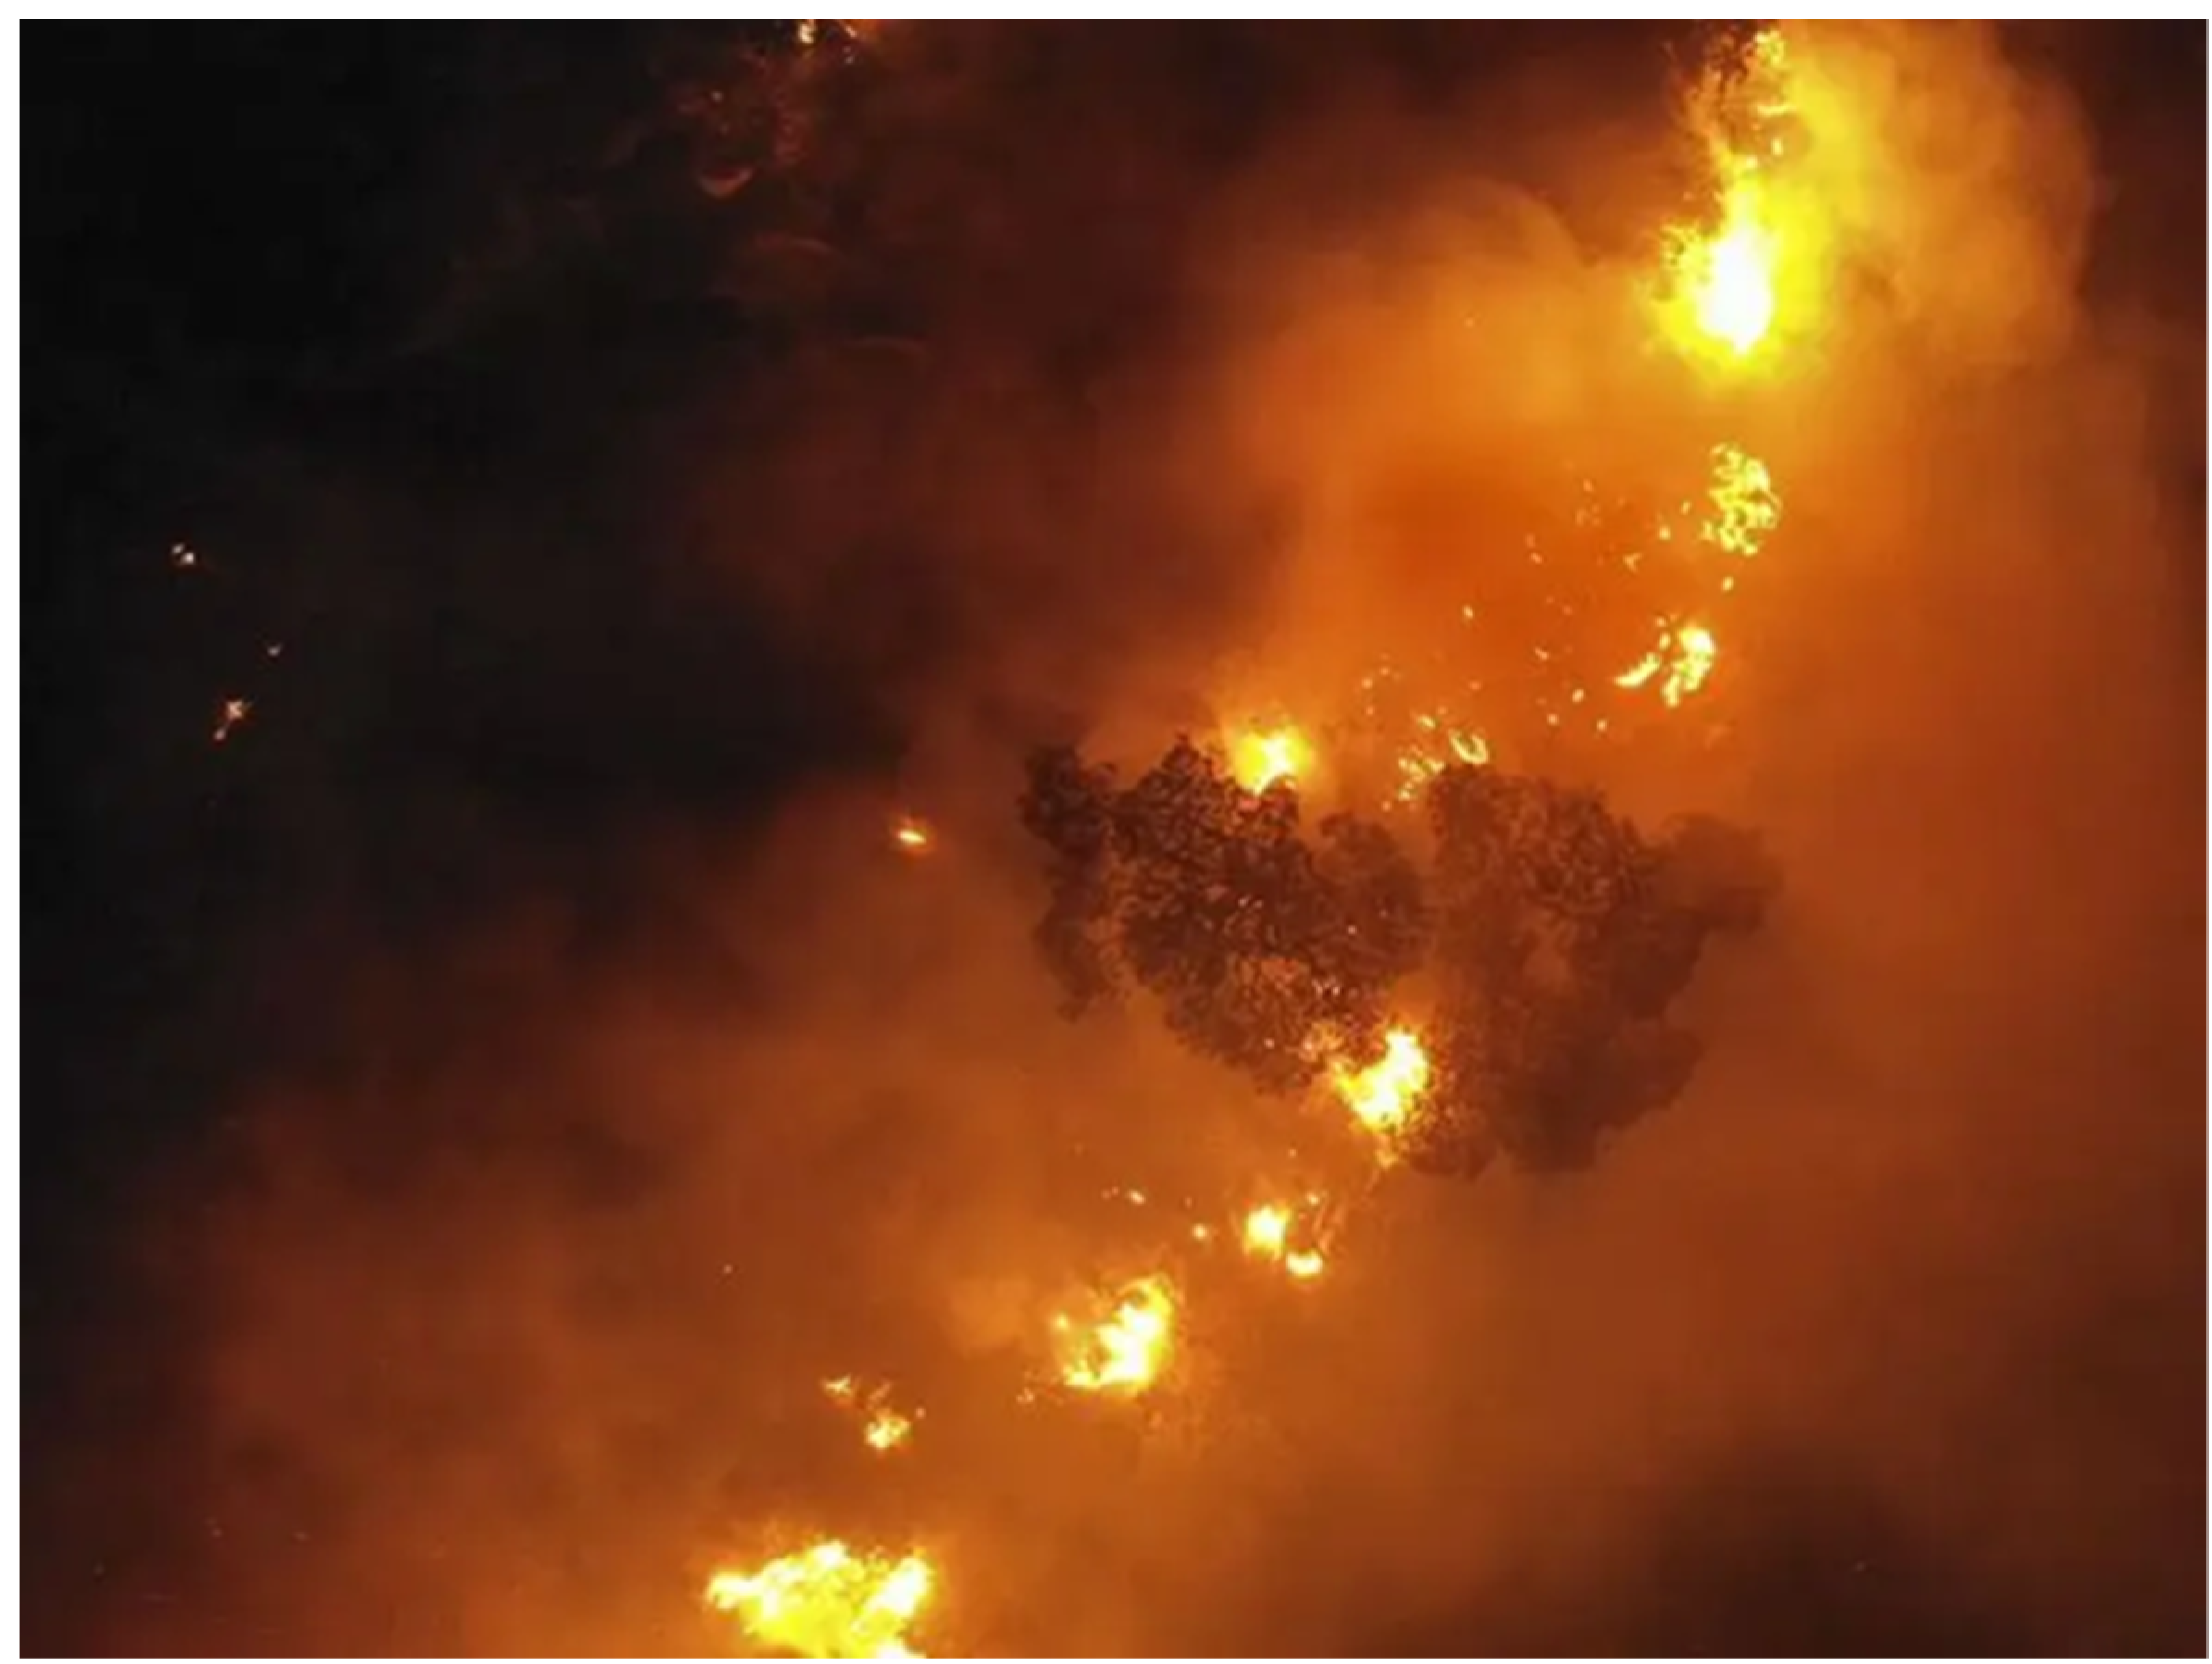
\includegraphics[width=0.2\textwidth]{wildfire.png}
\caption{A photo of a sunset via Adrian Pelletier}
\centering
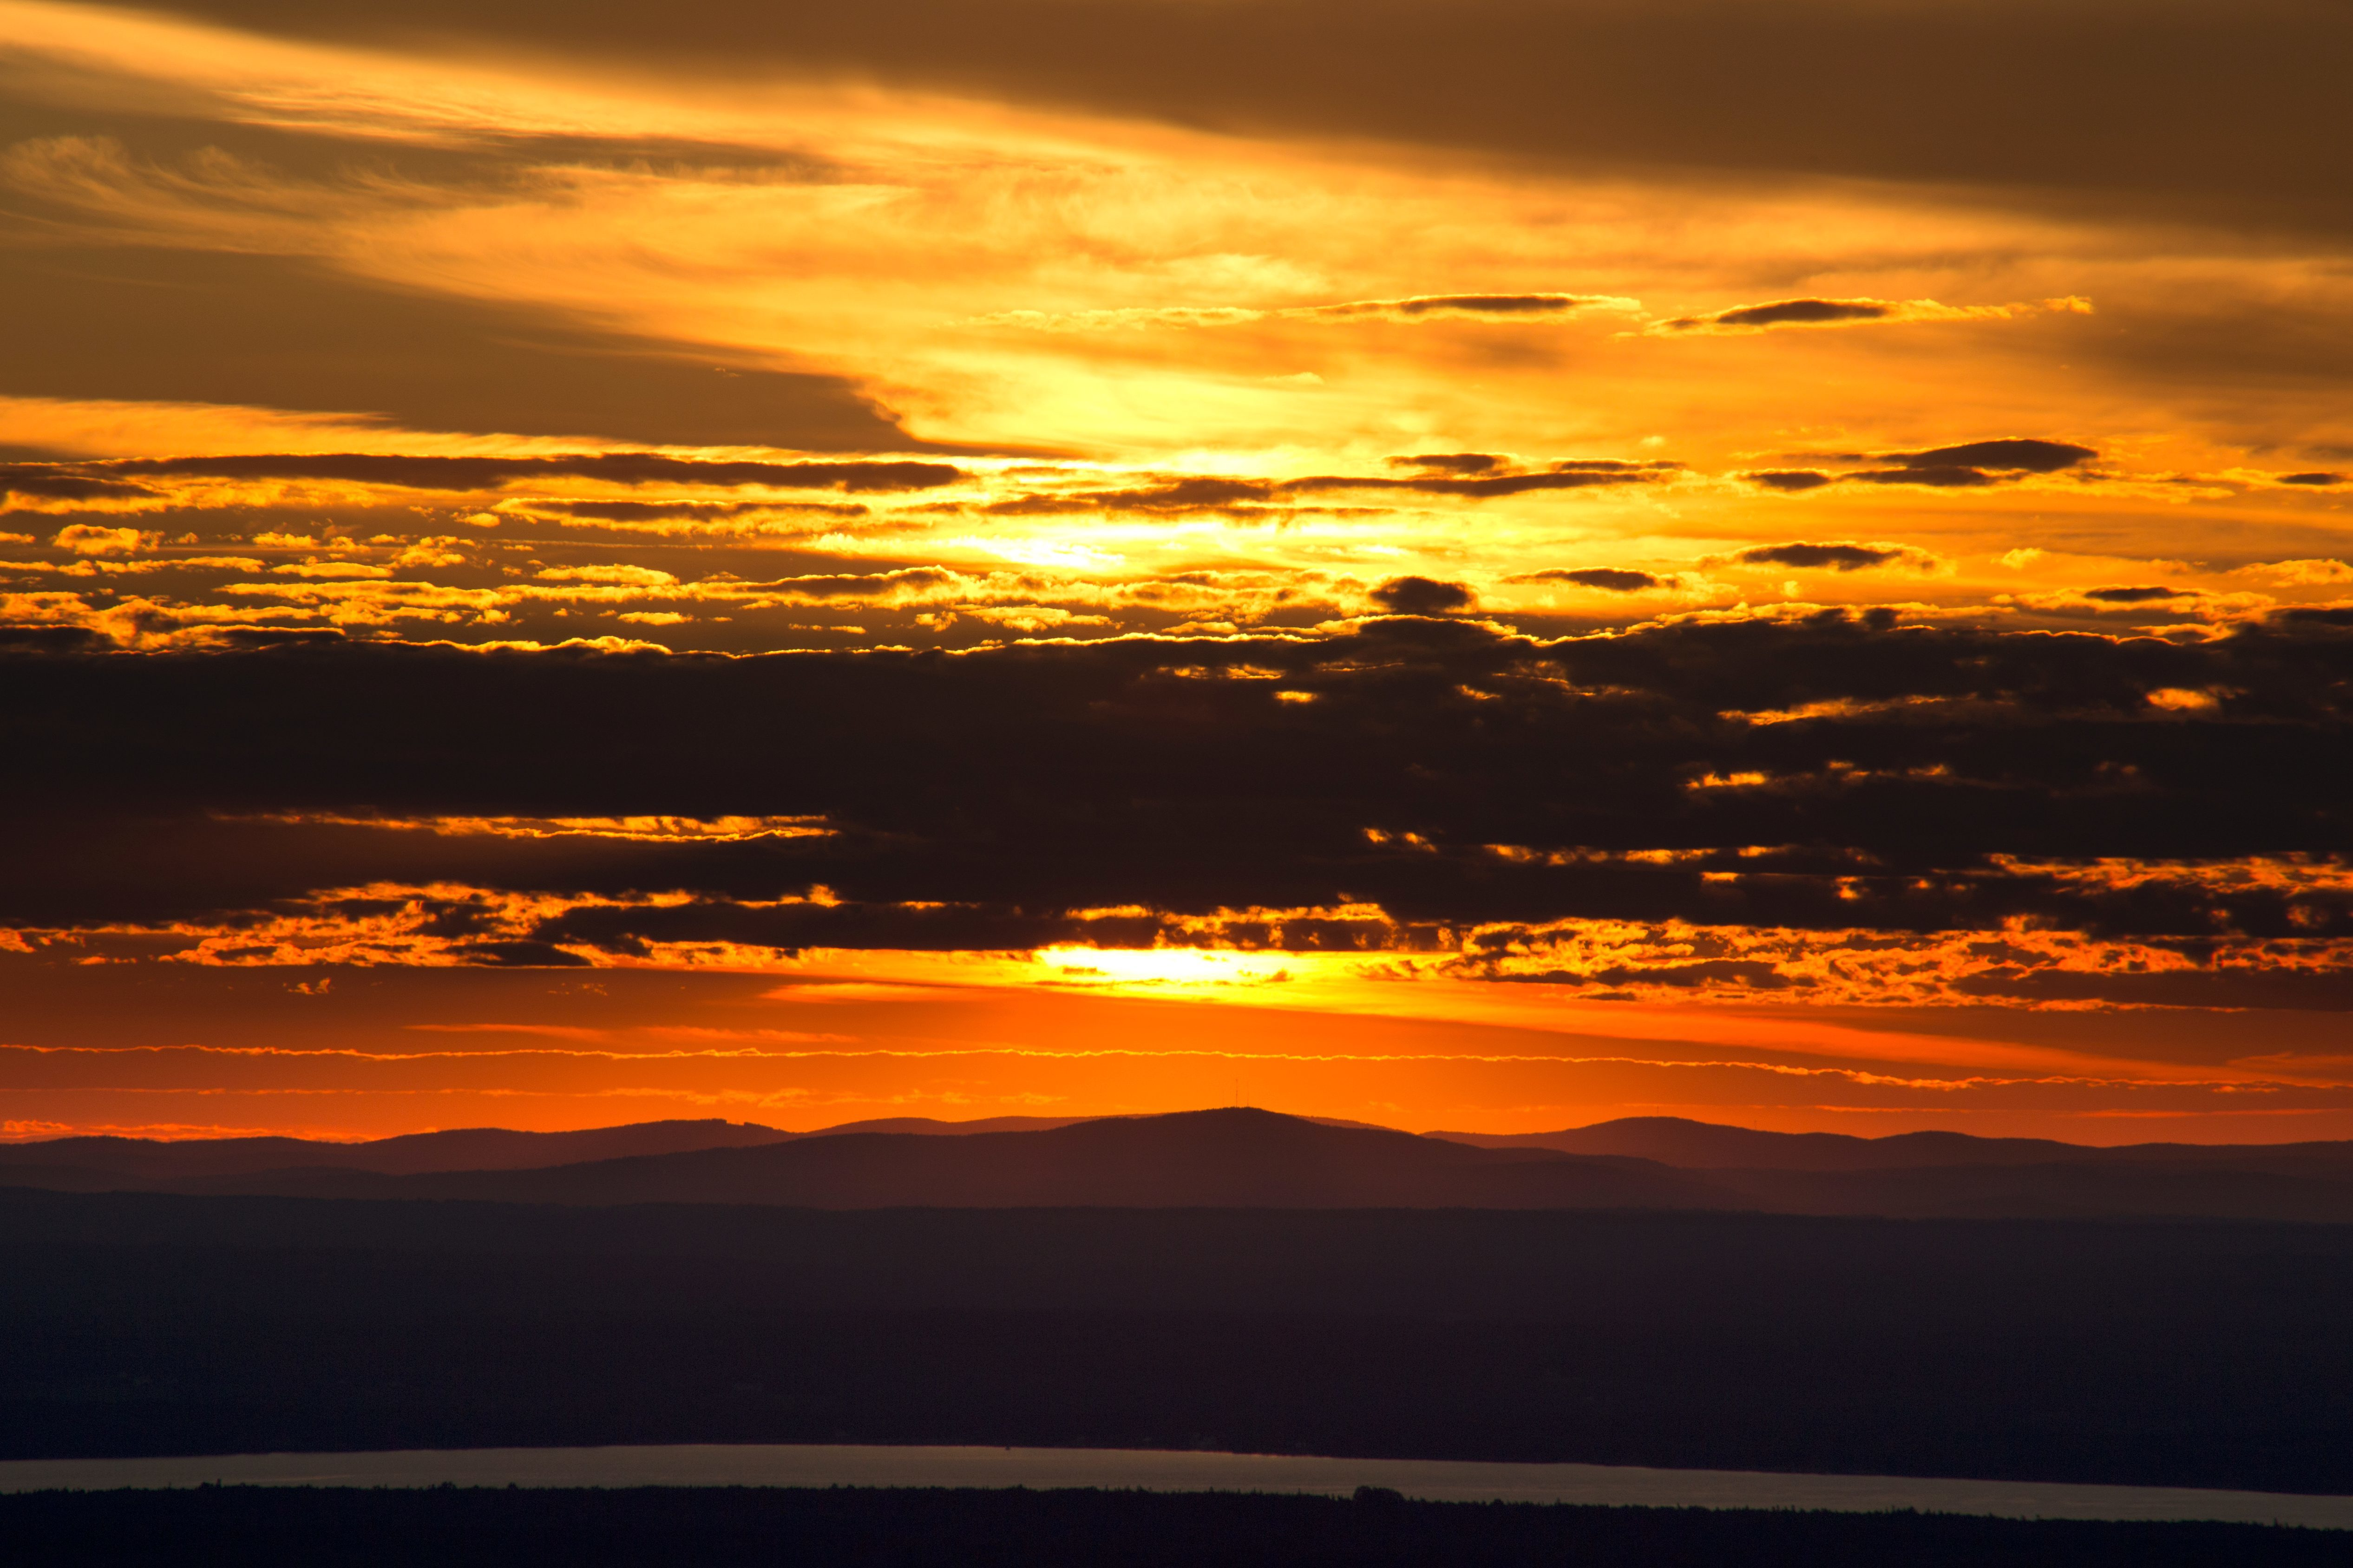
\includegraphics[width=0.2\textwidth]{sunset.jpg}
\end{figure}

\section{Motivation}
Ours is not the only wildfire detection method to utilize machine learning. Last year, Google became a founding partner in the Earth Fire Alliance, which launched their wildfire detecting/tracking satellite, FireSat. However, FireSat is not a very accessible solution for potential clients. Beyond requiring a specially-designed satellite, FireSat’s detection method relies on pre-captured imagery of the desired location \cite{FireSat}. Other solutions eschew a single robust sensor for a robust network of sensors. However, deploying a network of temperature sensors across a forest presents its own challenges. Bindal et al. note that their system struggles to adapt to new environments and real-world variation [2024]. For instance, a network trained on temperatures from British Columbia may not function the same if deployed in, say, Brazil.
 
Therefore, the principle benefits offered by our solution are accessibility and adaptability. Our solution can function with only a single, simple sensor (i.e., a camera). However, it can still be scaled to utilize a network of sensors, like Bindal et al.’s proposed system; or it could be adapted to supplement an existing solution like FireSat. Google is already interested in reducing FireSat’s margin of error by checking against nearby infrastructure and local weather \cite{FireSat}. Our solution could become a part of that error-checking process.

\section{Problem Definition}

Given a corpus $M$ of aerial forest wildfire images and a single image $x \in M$, our task is to learn a mapping function $f(x) \colon M \to L$. This function maps the input image to a discrete set of multi-class risk categories, defined as $L = \{\text{Low}, \text{Medium}, \text{High}\}$. By evaluating the visual features of $x$, the function outputs the corresponding risk level $l \in L$, aiming to minimize false positives caused by confounding environmental elements such as terrain, weather, amount of foliage, etc.

\bibliographystyle{ACM-Reference-Format}
\begin{thebibliography}{9}
\bibitem{El-Madafri}
Ismail El-Madafri, Marta Peña, and Noelia Olmedo-Torre. 2023. The Wildfire Dataset: Enhancing Deep Learning-Based Forest Fire Detection with a Diverse Evolving Open-Source Dataset Focused on Data Representativeness and a Novel Multi-Task Learning Approach. \emph{Forests} 14, Article 9 (August 2023) https://doi.org/10.3390/f14091697
\bibitem{FireSat}
Molly McHugh-Johnson. 2025. Inside the launch of FireSat, a system to find wildfires earlier. Retrieved from https://blog.google/innovation-and-ai/products/inside-firesat-launch-muon-space/
\bibitem{Bindal}
Rohi Bindal, Shubhangi Deokar, Trilochan Singh Rathore, Aditi Sharma, Rupali Gangarde, and Ashwini Jatti. 2024. AI-ML Innovations in Forest Fire Detection: Protecting Ecosystems and Communities. In \emph{2024 International Conference on Computing, Sciences and Communications (ICCSC)} October 24 - 25, 2024, Ghaziabad, India. 10.1109/ICCSC62048.2024.10830309
\end{thebibliography}

\end{document}
